
\documentclass[9pt,a4paper,twoside]{tau}
% \usepackage[spanish,es-nodecimaldot,es-noindentfirst]{babel}
\usepackage[english]{babel}
\usepackage{graphicx}
\usepackage{tau}
\usepackage{float}
\usepackage{multicol}

%----------------------------------------------------------
% Title
%----------------------------------------------------------

\title{Custom CPU Architecture: ARM Cortex M0 implementation}

%----------------------------------------------------------
% Authors, affiliations and professor
%----------------------------------------------------------

\author[a]{David Ortiz Cota}
\author[a]{Sebastián Pulido Espinoza}
\author[a]{Alfredo Romo}
\author[a]{Jorge González Díaz}

%----------------------------------------------------------

\affil[a]{Student}
% \affil[b]{Affiliation of author two}
% \affil[c]{Affiliation of author three}

\professor{José Ignacio Parra Vilchis}

%----------------------------------------------------------
% Footpage notes
%----------------------------------------------------------

\institution{Tec de Monterrey, Campus Guadalajara}
\ftitle{}
\date{Jun 5, 2024}
\etal{}
\course{System on Chip Design}

%----------------------------------------------------------
% Abstract
%----------------------------------------------------------

\begin{abstract}    
    This paper delves into the intricate design and implementation of a complete microprocessor based on the ARM Cortex M0 Harvard architecture. Moving beyond a single instruction, it explores the fundamental building blocks that orchestrate the complex process of fetching, decoding, and executing instructions. The paper outlines the core architecture of the microprocessor, including the key functional units like the Control Unit, Arithmetic Logic Unit (ALU), Program Memory, register file and RAM. It delves into the instruction set architecture (ISA), detailing the instruction formats, addressing modes, and their impact on program execution. The implementation details encompass the logic design principles employed for each unit, exploring the data flow and control signals that govern their operation. Furthermore, the paper discusses the memory hierarchy and its interaction with the processor.\\
    Finally, the paper touches upon the challenges encountered during implementation, potential optimization strategies, and the verification methodologies used to ensure the microprocessor's functionality. This comprehensive exploration provides valuable insights into the intricate world of microprocessor design, serving as a valuable resource for computer architecture students and professionals.
\end{abstract}

%----------------------------------------------------------

\keywords{Arm Cortex M0, Harvard, Microcontroller, Microprocessor, Verilog, FPGA board, Hardware Description Language, Soft processor}

%----------------------------------------------------------

\begin{document}
	
    \maketitle
    \thispagestyle{firststyle}
    \abscontent
    \tableofcontents

%----------------------------------------------------------


%----------------------------------------------------------%
%%                   INTRODUCTION                         %%
%----------------------------------------------------------%
\section{Introduction}

    \taustart{M}icroprocessors, the brains of modern computing devices, orchestrate the complex dance of data processing that powers our digital world. This paper embarks on a journey to unravel the intricacies of microprocessor design and implementation, delving into the fundamental principles that govern these remarkable machines.

    A microprocessor is a computer processor for which the data processing logic and control is included on a single integrated circuit (IC), or a small number of ICs. The microprocessor contains the arithmetic, logic, and control circuitry required to perform the functions of a computer's central processing unit (CPU). The IC is capable of interpreting and executing program instructions and performing arithmetic operations. The microprocessor is a multipurpose, clock-driven, register-based, digital integrated circuit that accepts binary data as input, processes it according to instructions stored in its memory, and provides results (also in binary form) as output. Microprocessors contain both combinational logic and sequential digital logic, and operate on numbers and symbols represented in the binary number system.

    \subsection{Brief History of Microprocessors.}
    It all began with the invention of the transistor by Bell Labs in the 1950s. These tiny, solid-state devices replaced bulky and power-hungry vacuum tubes, paving the way for smaller and more efficient electronic circuits. This technological leap laid the foundation for the integrated circuit (IC), a revolutionary concept conceived by Jack Kilby at Texas Instruments (TI) in 1958. The IC miniaturized electronics even further by integrating multiple transistors onto a single silicon chip, dramatically reducing size and complexity. \\
    The year 1971 witnessed the birth of the first commercially available microcontrollers. There's some debate about which device holds this title. The Texas Instruments TMS 1000, developed by Gary Boone and Michael Cochran, is widely recognized as a pioneer. This 4-bit microcontroller had a simple instruction set, built-in memory, and rudimentary input/output (I/O) capabilities, making it suitable for basic control tasks. Around the same time, Intel released its 4-bit 4004. Initially designed for calculators, the 4004's versatility and low cost led to broader applications in control systems. These early microcontrollers marked the beginning of a new era in embedded computing.

    \subsection{Existing Architectures}
    There are 2 main existing architectures used nowadays, they are Von Neumann Architecture and Harvard Architecture.

        \subsubsection{Hardvard Architecture:}
        The Harvard architecture is a computer architecture with separate storage and signal pathways for instructions and data. It is often contrasted with the von Neumann architecture, where program instructions and data share the same memory and pathways. This architecture is often used in real-time processing or low-power applications.
        There is no need to make the two memories share characteristics. In particular, the word width, timing, implementation technology, and memory address structure can differ. In some systems, instructions for pre-programmed tasks can be stored in read-only memory while data memory generally requires read-write memory. In some systems, there is much more instruction memory than data memory so instruction addresses are wider than data addresses.
    
        \subsubsection{Von Neumann Architecture}
        The von Neumann architecture is a foundational design concept for computers. It features a unified memory space that stores both program instructions and data. The CPU fetches both from this single location, simplifying the overall design and control logic. This architecture typically involves sequential access, where instructions and data are retrieved one after another. While this can be efficient for applications where instruction and data access are balanced, it can create bottlenecks for tasks requiring frequent data manipulation, as the CPU might need to wait for data retrieval before continuing program execution. Despite this potential drawback, the von Neumann architecture remains popular due to its simplicity, ease of programming, and cost-effectiveness, making it a suitable choice for general-purpose computing.

        \subsubsection{Dataflow Architecture}
        Dataflow architecture is a dataflow-based computer architecture that directly contrasts the traditional von Neumann architecture or control flow architecture. Dataflow architectures have no program counter, in concept: the executability and execution of instructions is solely determined based on the availability of input arguments to the instructions, so that the order of instruction execution may be hard to predict.\\

        Although no commercially successful general-purpose computer hardware has used a dataflow architecture, it has been successfully implemented in specialized hardware such as in digital signal processing, network routing, graphics processing, telemetry, and more recently in data warehousing, and artificial intelligence (as: polymorphic dataflow Convolution Engine, structure-driven, dataflow scheduling). It is also very relevant in many software architectures today including database engine designs and parallel computing frameworks.

        Synchronous dataflow architectures tune to match the workload presented by real-time data path applications such as wire speed packet forwarding. Dataflow architectures that are deterministic in nature enable programmers to manage complex tasks such as processor load balancing, synchronization and accesses to common resources.

        \subsubsection{Vector Architecture}
        A vector processor or array processor is a central processing unit (CPU) that implements an instruction set where its instructions are designed to operate efficiently and effectively on large one-dimensional arrays of data called vectors. This is in contrast to scalar processors, whose instructions operate on single data items only, and in contrast to some of those same scalar processors having additional single instruction, multiple data (SIMD) or SWAR Arithmetic Units. Vector processors can greatly improve performance on certain workloads, notably numerical simulation and similar tasks. Vector processing techniques also operate in video-game console hardware and in graphics accelerators.

        
        




    
    \subsection{Existing implementations}
    There also 2 main existing implementations, they are the Complex Instruction Set Computer (CISC) and Reduced Instruction Set Computer (RISC). An instruction set, also known as an Instruction Set Architecture (ISA), is essentially the language a processor understands. It defines a set of commands that the processor can execute to perform various operations. These operations can be simple, like adding two numbers, or more complex, like moving data between memory locations or controlling external devices.

        \subsubsection{RISC}
        RISC processors focus on a smaller set of simpler instructions. These instructions typically perform a single, well-defined operation. While they might require more instructions to achieve the same result as a single CISC instruction, their simplicity allows for faster execution and optimization. RISC processors often excel in performance due to their simpler instructions. These instructions can be decoded and executed more efficiently, leading to faster processing speeds.
        Well-known RISC architectures include ARM (used in most mobile devices) and SPARC (developed by Oracle).

        \subsubsection{CISC}
        CISC processors boast a rich set of complex instructions. These instructions can perform multiple operations in a single step, making programming potentially easier and more intuitive for developers. For example, a single CISC instruction might add two numbers and store the result in a specific memory location. While CISC instructions can be efficient for some tasks, their complexity can sometimes lead to slower execution compared to RISC. Decoding these complex instructions can take time, and they might not always be perfectly optimized for the hardware. Popular CISC architectures include the x86 family (used by Intel and AMD) and the POWER architecture (developed by IBM).


        \subsubsection{VLIW}
        Very long instruction word refers to instruction set architectures that are designed to exploit instruction-level parallelism (ILP). A VLIW processor allows programs to explicitly specify instructions to execute in parallel, whereas conventional central processing units (CPUs) mostly allow programs to specify instructions to execute in sequence only. VLIW is intended to allow higher performance without the complexity inherent in some other designs.

        The traditional means to improve performance in processors include dividing instructions into substeps so the instructions can be executed partly at the same time (termed pipelining), dispatching individual instructions to be executed independently, in different parts of the processor (superscalar architectures), and even executing instructions in an order different from the program (out-of-order execution). These methods all complicate hardware (larger circuits, higher cost and energy use) because the processor must make all of the decisions internally for these methods to work.

        In contrast, the VLIW method depends on the programs providing all the decisions regarding which instructions to execute simultaneously and how to resolve conflicts. As a practical matter, this means that the compiler (software used to create the final programs) becomes more complex, but the hardware is simpler than in many other means of parallelism.

    \subsection{Our Implementation}
    The implementation that we well be looking into in the following steps of this paper is a Hardvard architecture, ARM Cortex M0 - based microprocessor with a custom \textit{Instuction Set Architecture} (ISA). 
    This implementation, although simple, is still fairly complete and powerfull, as it has the basic functionality of any general pourpose computer and the  \textit{ISA} is based on the simplest but complete architecture ARM has to offer. Our ISA (touched upon later in this paper) consist of 4 byte encodings(32 bit) based on the 32 bit  \textit{Thumb-2} ISA that is used in most Cortex M and similar microcontrollers.
    
    

%----------------------------------------------------------%
%%                   Design & implementation              %%
%----------------------------------------------------------%
\section{Design and Implementation}
    As previously mentioned, our architecture is based on an Arm Cortex M0 3-stage architecture. \\
    The 3-stage pipeline is a fundamental concept in computer architecture that optimizes the instruction processing speed within a CPU. It breaks down the instruction execution process into three distinct stages, allowing the CPU to work on multiple instructions simultaneously.\\
\subsection{Pipeline overview}
    \begin{itemize}
        \item 1. Fetch (Instruction Fetch):
        In this stage, the CPU fetches an instruction from memory based on the address provided by the program counter (PC). Think of it like a librarian retrieving a book (instruction) from the shelf (memory) based on the call number (PC).
        \item 2. Decode (Instruction Decode): Once fetched, the instruction is passed to the decode stage. Here, the control unit deciphers the instruction by analyzing its opcode (operation code) and operands.
        Imagine the librarian decoding the Dewey Decimal System (opcode) and identifying the section (data to be processed) and category (operation) of the book (instruction).
        \item 3. Execute (Instruction Execution): In the final stage, the decoded instruction is executed. The control unit sends control signals to the relevant ALU (Arithmetic Logic Unit) or other execution units based on the instruction type (addition, data transfer, etc.). The ALU performs the designated operation and stores the result. This stage is like the librarian following the instructions (data and operation) in the book (instruction) to perform a specific task (calculation, data movement).
    
    \end{itemize}
    

\begin{figure}[h]  % The [h] here is a placement specifier (here)
    \centering  % This command centers the image
    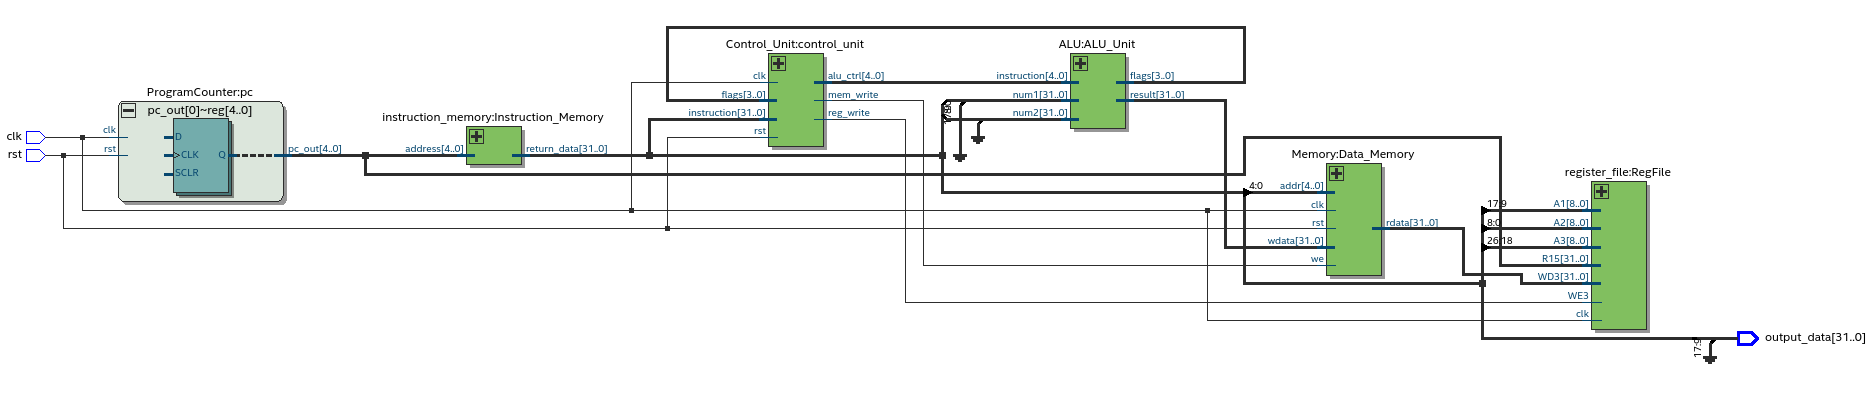
\includegraphics[width=0.5\textwidth]{images/RTLImg.png}
    \caption{RTL Overview}
    \label{fig:RTL Overview}
\end{figure}

%----------------------------------------------------------%
%%                   
%%                      Modules
%%
%----------------------------------------------------------%




\subsection{Modules}
There are 5 main modules that form the CPU, the \textit{Program Counter}, \textit{Instruction Memory}, \textit{ALU}, \textit{Data Memory}, \textit{Register File}.\\ Each one of them will be explained in detail, as well as there individual inputs and outputs:

%----------------------------------------------------------%
%%                   PROGRAM COUNTER
%----------------------------------------------------------%
\subsubsection{PC}
    The program counter (PC), also known as instruction pointer (IP), is a critical register within the CPU of a microprocessor. It acts like a conductor's baton, keeping track of the memory address from which the next instruction will be fetched. In essence, the PC dictates the execution flow of a program by specifying the sequence of instructions to be processed by the CPU.

    The value of the program counter can be modified to allow for \textit{jumps} and \textit{branches} (which have yet to be implemented in our architecture). In our PC implementation, the program counter starts and resets at 0, and count up by 1 every clock cicle.\\
    
    \textbf{Inputs}:
    \begin{itemize}
        \item Clock and Reset: the value PC value increments by 1 every clock cicle and resets to 0 when the reset signal is enabled 
    \end{itemize}
    \textbf{Outputs}:
    \begin{itemize}
        \item PC Value: the actual value of the PC, will be the address of the instruction retrieved from the \textit{Instruction Memory}.
    \end{itemize}
    
    \begin{figure}[h]  % The [h] here is a placement specifier (here)
        \centering  % This command centers the image
        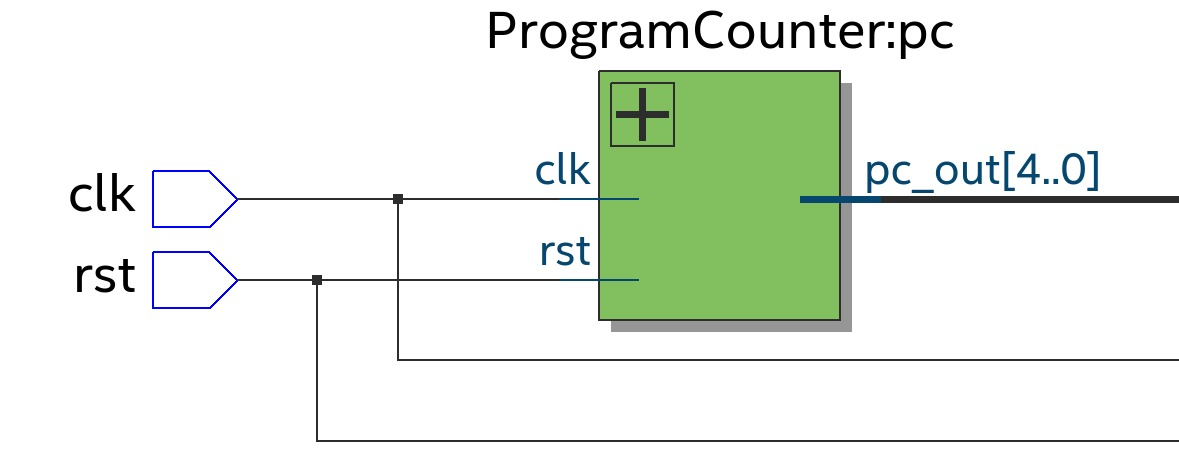
\includegraphics[width=0.3\textwidth]{images/PCImg.png}
        \caption{Program Counter RTL}
        \label{fig:Counter RTL}
    \end{figure}





%----------------------------------------------------------%
%%                   INSTRUCTION MEMORY
%----------------------------------------------------------%
\subsubsection{Instruction Memory}
    The instruction memory module, often abbreviated as IM, serves as the brain's storage room for a program's instructions within a microprocessor. It's a read-only memory (ROM) specifically designed to hold the sequence of instructions that make up the software being executed. \\

    The main functions of the Instruction Memory are the following:

    \begin{itemize}
        \item \textbf{Storage}: The IM stores the program code in the form of binary machine code instructions. These instructions are pre-loaded before program execution and remain fixed throughout.
        \item \textbf{Retrieval}: When the program counter sends a memory address, the instruction memory acts like a lookup table. It retrieves the instruction located at that specific address.
        \item \textbf{Feeding the Pipeline}: The retrieved instruction is then fed into the processor's pipeline for decoding and execution. This fetch-decode-execute cycle continues until the program terminates.\\
    \end{itemize}

    \textbf{Inputs}:
    \begin{itemize}
        \item Address: Program counter output (interpreted as the address to retrieve from memory).

    \end{itemize}
    
    \textbf{Outputs}:
    \begin{itemize}
        \item Instruction: 32-bit instruction retrieved from memory.
    \end{itemize}


    \begin{figure}[h]  % The [h] here is a placement specifier (here)
        \centering  % This command centers the image
        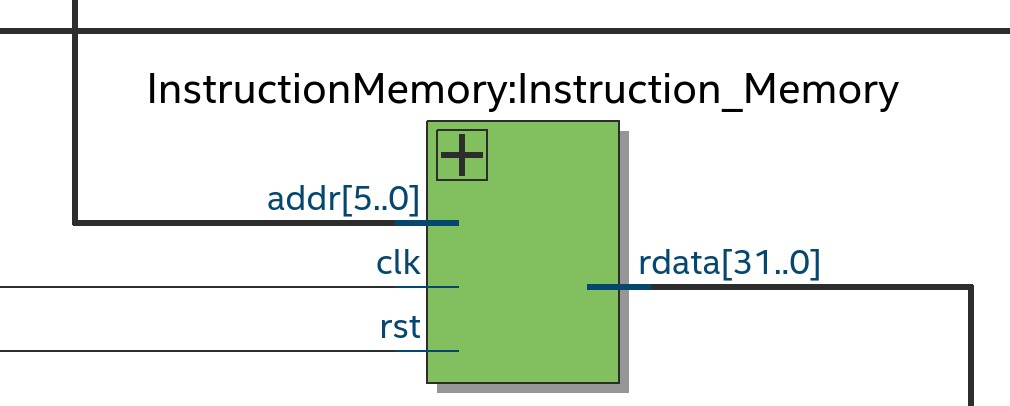
\includegraphics[width=0.5\textwidth]{images/InstMemImg.png}
        \caption{Instruction Memory RTL}
        \label{fig:Instruction Memory RTL}
    \end{figure}
    
%----------------------------------------------------------%
%%                   CONTROL UNIT
%----------------------------------------------------------%
\subsubsection{Control Unit}
    The control unit (CU) acts as the conductor of the orchestra within a microprocessor's central processing unit (CPU). It's the central brain that interprets instructions, coordinates execution, and ensures all the other parts work together seamlessly. The details of its operation are the following:

    \begin{itemize}
        \item \textbf{Instruction Decoding}: Once fetched, the CU decodes the instruction to understand the operation it represents. This involves deciphering the binary code of the instruction and identifying what needs to be done, it takes the first 5 bits of the instruction and interprets it as an OPCODE, the remaining bits are interpreted as \textit{destination} for the selected operation (9-bits), and operands 1 \& 2 (9-bits and 9-bits).
        
        \item \textbf{Issuing Control Signals}: Based on the decoded instruction, the CU generates control signals that act like instructions for other CPU components. These signals direct the arithmetic logic unit (ALU) to perform calculations, tell registers where to store data, and coordinate communication with memory and input/output devices.
        
        \item \textbf{Execution Flow Management}: The CU doesn't just issue commands; it also manages the overall flow of program execution. It determines the sequence of steps involved in executing an instruction and ensures they happen in the correct order. This might involve fetching operands (data to be manipulated), sending them to the ALU, and then storing the results. \\ 

    \end{itemize}

    \textbf{Inputs}:
    \begin{itemize}
        \item Clk and Rst: Clock and reset signals.
        \item Instruction: 32-bit instruction received from Instruction  Memory.
        \item Flags: flags recieved from a previous ALU operation.
    \end{itemize}
    
    \textbf{Outputs}:
    \begin{itemize}
        \item Memory to Register: Enables whether the memory output should be written to registers.
        \item Memory Write Enable: Write enable signal for Data Memory
        \item Alu Control: 5 bit OPCODE for ALU in case the instruction requires it
    \end{itemize}
    


    \begin{figure}[h]  % The [h] here is a placement specifier (here)
        \centering  % This command centers the image
        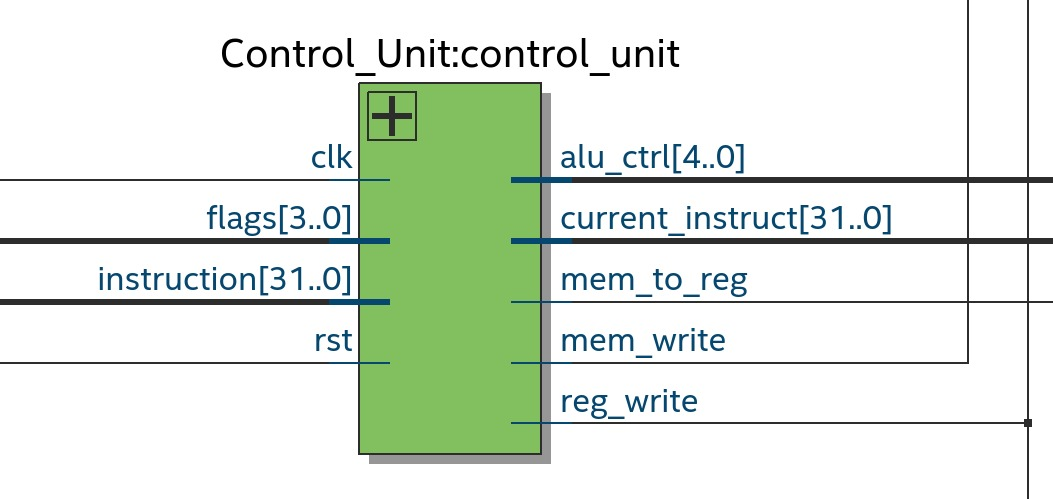
\includegraphics[width=0.3\textwidth]{images/CUImg.png}
        \caption{Control Unit RTL}
        \label{fig:Control Unit RTL}
    \end{figure}



%----------------------------------------------------------%
%%                   ALU
%----------------------------------------------------------%
\subsubsection{ALU}
    The ALU, which stands for Arithmetic Logic Unit, is the workhorse of the CPU (Central Processing Unit)  when it comes to performing calculations and making logical decisions. It can do arithmetic operation like addition and subtraction, Logical operations like comparing 2 numbers, and bitwise operations like shifts\\ \\

    \textbf{Inputs}:
    \begin{itemize}
        \item Instruction: 5-bit OPCODE that gets interpreted as a certain operation via a demultiplexer.
        \item Num1 \& Num2: Operands for operations
    \end{itemize}
    
    \textbf{Outputs}:
    \begin{itemize}
        \item Flags: Flags raised by certain operations. Our architecture includes flags for \textit{Negative, Zero, Carry \& oVerflow}
        \item Result: 32-bit result from whatever operation was performed by the Alu.
    \end{itemize}
    



    \begin{figure}[h]  % The [h] here is a placement specifier (here)
        \centering  % This command centers the image
        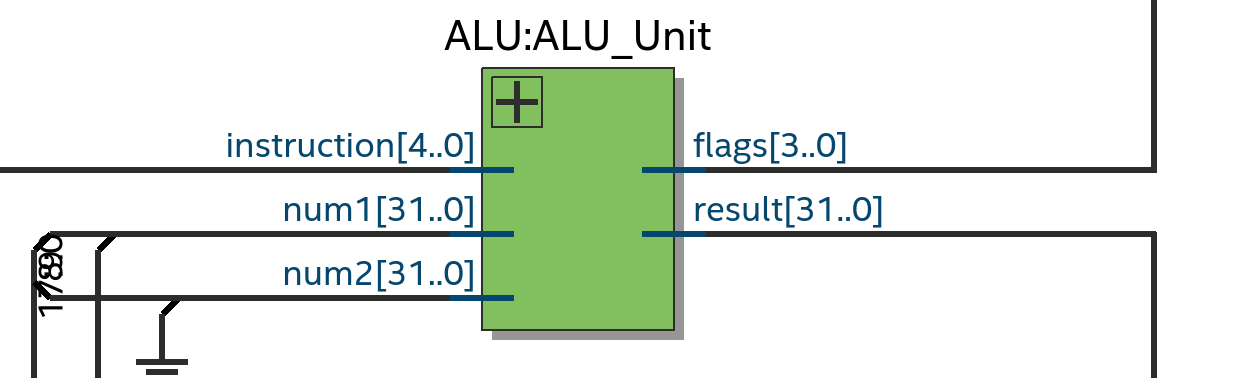
\includegraphics[width=0.5\textwidth]{images/ALUImg.png}
        \caption{ALU RTL}
        \label{fig:ALU RTL}
    \end{figure}


%----------------------------------------------------------%
%%                   DATA MEMORY
%----------------------------------------------------------%
\subsubsection{Data Memory}
    Data memory, also commonly referred to as RAM (Random Access Memory), is the work area of a microprocessor where it stores and retrieves the temporary data that's actively used during program execution. Unlike instruction memory, which holds the program instructions permanently, data memory is constantly changing as the program progresses. It serves as the temporary storage space for various types of data, including:
    Variables, Intermediate Results, Function Arguments, Return Values and Heap Memory.\\
    Data memory is volatile, meaning it loses its content when the power is turned off. This is because RAM uses capacitors to store data, and these capacitors discharge over time without a constant power supply.\\

    \textbf{Inputs}:
    \begin{itemize}
        \item Clk and Rst: When the rst signal is active, the memory resets to all 0's.
        \item we: Write enable to determin read or write operation.
        \item wdata: Data to be written to a certain memory address (in case write enable is active).
        \item Address: Address to be writen or retrieved from memory.
    \end{itemize}
    
    \textbf{Outputs}:
    \begin{itemize}
        \item Return Data: If write enable is disabled, the data fetched will be returned via this bus.
    \end{itemize}


    \begin{figure}[h]  % The [h] here is a placement specifier (here)
        \centering  % This command centers the image
        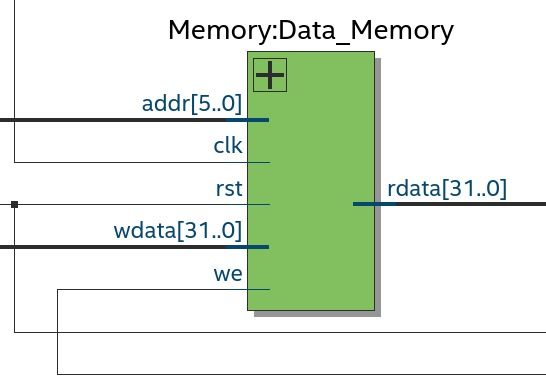
\includegraphics[width=0.3\textwidth]{images/DataMemImg.png}
        \caption{Data Memory RTL}
        \label{fig:Data Memory RTL}
    \end{figure}


%----------------------------------------------------------%
%%                   REGISTER FILE
%----------------------------------------------------------%
\subsubsection{Register File}


\begin{figure}[h]  % The [h] here is a placement specifier (here)
    \centering  % This command centers the image
    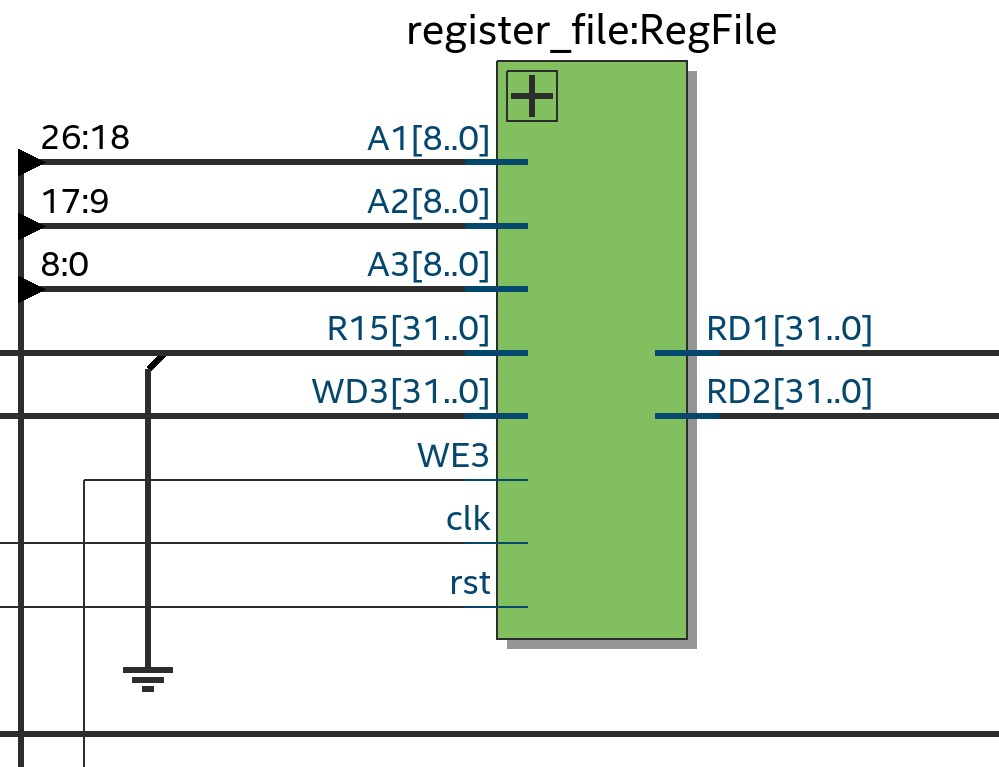
\includegraphics[width=0.27\textwidth]{images/RegFileImg.png}
    \caption{Register File RTL}
    \label{fig:Register File RTL}
\end{figure}


    The register file is a set of high-speed internal memory locations within the CPU (Central Processing Unit).  They act as the CPU's scratchpad or workbench, holding frequently accessed data and intermediate results for quick manipulation. Compared to main memory (data memory), registers offer significantly faster access times, making them critical for efficient program execution. \\
    This implementation consist of a 14+1 register file. The first 14 registers act general function registers, while the 15th register gets its value from the program counter + 2, the purpose of this offset is to compensate for the 2 clock cicles that have elapsed (Fetch/Decode) from the previous clock cicles.

    \textbf{Inputs}:
    \begin{itemize}
        \item Clk and Rst: When the rst signal is active, the memory resets to all 0's.
        \item A1 \& A2: Addresses to be acted upon, received from the instruction.
        \item A3: Writeback address.
        \item WE3: Write enable from address 3 (recieved from the Control Unit).
        \item R15: Value recieved from the program counter (+2 for reasons mentioned above).
    \end{itemize}
    
    \textbf{Outputs}:
    \begin{itemize}
    \item RD1 \& RD2: Return data from A1 and A2, used as the operands for the ALU.
    \end{itemize}
    



       %----------------------------------------------------------%
        %%                   Opcode description                   %%
        %----------------------------------------------------------%
        \section{Custom Instruction Set Architecture}

        Our custom \textit{Instruction Set Architecture} (ISA) is based on the 32 bit (4 byte) Thumb-2 ISA. The main difference regarding our ISA is that the Thumb-2 instructions are generally stored on contigous 8 bit blocks of memory while our ISA consists of a block of 32 bit instructions.\\

        Out of these 32 bits, the first 5 of them are intended to be used as the instruction opcode which identifies the type of operation that will be executed, leaving us with 27 free bits which will be distributed equally for specifying destination and source memory addresses for instruction execution. 
        We propose using a total of 18 instructions that run inside the ALU. These instructions span from simple logical operations like an AND bitwise instruction operation, to arithmetic operations like adding of two integers. We \textit{do not implement floating point arithmetic} natively. If Floating Point Arithmetic is requierd it would need to be managed by software. 

        \subsection{Opcode}

        \begin{figure}[h]  % The [h] here is a placement specifier (here)
            \centering  % This command centers the image
            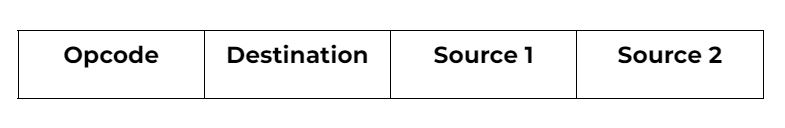
\includegraphics[width=0.5\textwidth]{images/ISA.JPG}
            \caption{Instruction Set Format}
            \label{fig:ISA Format}
        \end{figure}

        The main consideration for designing and understanding the opcode of our proposed architecture is knowing how many instructions there are to be represented. Adding up 18 operations from the ALU, 3 from the memory interactions, and 3 from jump instructions, we come out to needing 5 bits of opcode, given by the formula:
        \begin{equation}
            \text{Bits} = \left\lceil \log_{2}{x} \right\rceil
        \end{equation}
    



        % INSTRUCTION SET
        \section{ALU Instructions}

        The folowing instructions are executed by the \textit{Arithmetic Logic Unit} as they requiere math, logic, bitwise operations and comparisons:
    
        \subsection{ANDS}
        This operation performs a bitwise AND on two 32-bit operands, where each bit of the output is the logical AND of the corresponding bits of the operands. This means that if both corresponding bits are 1, then the output bit is 1, otherwise it is 0. 
        \subsection{ORRS}
        This operation performs a bitwise OR on two 32-bit operands, where each bit of the output is the logical OR of the corresponding bits of the operands. This means that if either corresponding bit is 1, then the output bit is 1, otherwise it is 0. 
        \subsection{MVNS}
        This operation performs a bitwise NOT on a 32-bit operand, which means that it flips all the bits of the operand. This is also known as a bitwise complement. 
        \subsection{EORS}
        This operation performs a bitwise XOR on two 32-bit operands, where each bit of the output is the logical XOR of the corresponding bits of the operands. This means that if the corresponding bits are not equal, then the output bit is 1, otherwise it is 0. 
        \subsection{ADCS}
        This operation performs an addition with carry on two 32-bit operands, where the carry flag is taken into account. This means that if the carry flag is set, then it is added to the result of the addition. This operation is useful for implementing multi-word arithmetic. 
        \subsection{ADDS}
        This operation performs a normal addition on two 32-bit operands, without taking the carry flag into account. This operation is useful for adding two numbers together. 
        \subsection{SBCS}
        This operation performs a subtraction with carry on two 32-bit operands, where the carry flag is taken into account. This means that if the carry flag is set, then it is subtracted from the result of the subtraction. This operation is useful for implementing multi-word arithmetic. 
        \subsection{SUB}
        This operation performs a normal subtraction on two 32-bit operands, without taking the carry flag into account. This operation is useful for subtracting two numbers together. 
        \subsection{MULS}
        This operation performs a multiplication on two 32-bit operands, where the result is a 32-bit value. This operation is useful for multiplying two numbers together. 
        \subsection{LSRS}
        This operation performs a logic shift right on a 32-bit operand, where the rightmost bit is shifted out, and the leftmost bit is filled with 0. This operation is useful for dividing a number by a power of 2. 
        \subsection{LSLS}
        This operation performs a logic shift left on a 32-bit operand, where the leftmost bit is shifted out, and the rightmost bit is filled with 0. This operation is useful for multiplying a number by a power of 2. 
        \subsection{ROR}
        This operation performs a rotate right on a 32-bit operand, where the rightmost bit is shifted into the leftmost bit and all other bits are shifted to the right. This operation is useful for circularly shifting a number. 
        \subsection{UXTB}
        This operation performs an unsigned extend byte on a 32-bit operand, where the lower 8 bits of the operand are sign-extended to 32 bits. This operation is useful for converting a byte value to a 32-bit value. 
        \subsection{UXTH}
        This operation performs an unsigned extend halfword on a 32-bit operand, where the lower 16 bits of the operand are sign-extended to 32 bits. This operation is useful for converting a halfword value to a 32-bit value. 
        \subsection{SXTB}
        This operation performs a signed extend byte on a 32-bit operand, where the lower 8 bits of the operand are sign-extended to 32 bits. This operation is useful for converting a byte value to a 32-bit value. 
        \subsection{SXTH}
        This operation performs a signed extend halfword on a 32-bit operand, where the lower 16 bits of the operand are sign-extended to 32 bits. This operation is useful for converting a halfword value to a 32-bit value. 
        \subsection{CMP}
        This operation performs a comparison between two 32-bit operands, where the result is determined by subtracting one operand from the other and setting the status flags based on the result. This operation is useful for comparing two numbers. 
        \subsection{NOP}
        This operation performs a no-operation, which means that it does nothing. This operation is useful for adding a delay or for synchronizing operations.
    
    
        %----------------------------------------------------------%
        %%                   Memory instructions                  %%
        %----------------------------------------------------------%
        \section{Memory instructions}
        This instructions don't require the use of the \textit{ALU}, they only move data around from one place (like the RAM) to another (Register File):
    
        \subsection{LOADI}
        This instruction loads data from memory (RAM) into a register. It is useful for accessing data stored in memory. 
        \subsection{STORE}
        This instruction stores data from a register into memory (RAM). It is useful for saving data to be used later.
        \subsection{Move (MOV)}
        This instruction moves data between registers or from a register to memory. It is useful for manipulating data within the processor.
    
        %----------------------------------------------------------%
        %%                    Jump instructions                   %%
        %----------------------------------------------------------%
        \section{Jump instructions}
        This instrcutions modify the normal flow of the program, they modify the data that the program counter uses to make it skip or move a certain number of instruction (sometimes only if a certain condition is met).
        
        \subsection{Jump (J)}
        This instruction allows the CPU to jump to a specific memory address to continue execution. It is useful for changing the flow of execution in a program. 
        \subsection{Branch Equal (BEQ)}
        This instruction enables the CPU to branch to a specific memory address if two registers are equal. It is useful for conditional branching in a program. 
        \subsection{Halt (HLT)}
        This instruction stops the CPU from executing further instructions, effectively halting the processor. It is useful for terminating a program or stopping execution when necessary.



        \begingroup
        {\centering
        \begin{tabular}{c|c}
        \textbf{Opcode} & \textbf{Operation} \\ \hline
        00000 & RESERVED \\
        00001 & ANDS \\
        00010 & ORRS \\
        00011 & MVNS \\
        00100 & EORS \\
        00101 & ADCS \\
        00110 & ADDS \\
        00111 & SBCS \\
        01000 & SUB \\
        01001 & MULS \\
        01010 & LSRS \\
        01011 & LSLS \\
        01100 & ROR \\
        01101 & UXTB \\
        01110 & UXTH \\
        01111 & SXTB \\
        10000 & SXTH \\
        10001 & CMP \\
        10010 & NOP \\
        10011 & LOADI \\
        10100 & STORE \\
        10101 & MOV \\
        10110 & J \\
        10111 & BEQ \\
        11000 & HLT \\
        11001-11111 & RESERVED \\
        \end{tabular}}


    
        
 

%\justifying
\section{Case of Study:}
    \subsection{Program description and Instructions}
    \subsection{C like code}

    \subsection{Data Flow}

    \subsection{Testbench \& results}


     
\section{Conclusion}
\justifying

CONCLUSION


%----------------------------------------------------------

\addcontentsline{toc}{section}{References}
\printbibliography

%----------------------------------------------------------

\end{document}

%---------------- Exmaple note and code -------------------
\begin{info}	
        Lorem ipsum dolor sit amet, consectetur adipiscing elit. Sed vestibulum justo quis massa aliquet, ut ultrices quam bibendum.
\end{info}